include(`macros.m4')

\pagebreak
\pdfbookmark[0]{process manipulation, program execution}{processes}

\begin{slide}
\sltitle{Contents}
\slidecontents{4}
\end{slide}

%%%%%%%%%%%%%%%%%%%%%%%%%%%%%%%%%%%%%%%%%%%%%%%%%%%%%%%%%%%%%%%%%%%%%%%%%

ifdef([[[NOSPELLCHECK]]], [[[
\pdfbookmark[1]{text/data/bss/stack/heap}{procmem}
]]])

\begin{slide}
\sltitle{Process memory layout in userspace}
\begin{center}
\begin{picture}(0,0)%
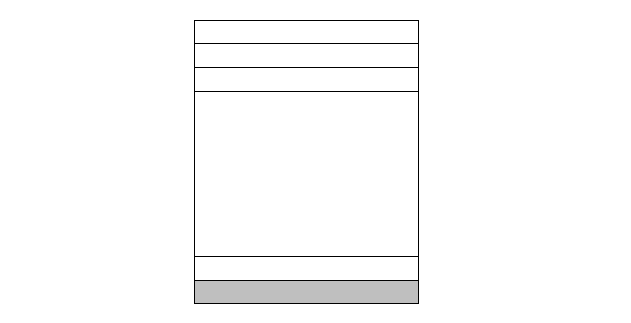
\includegraphics{img/tex/mem_user}%
\end{picture}%
\setlength{\unitlength}{4144sp}%
%
\begingroup\makeatletter\ifx\SetFigFont\undefined%
\gdef\SetFigFont#1#2#3#4#5{%
  \reset@font\fontsize{#1}{#2pt}%
  \fontfamily{#3}\fontseries{#4}\fontshape{#5}%
  \selectfont}%
\fi\endgroup%
\begin{picture}(4545,2184)(181,-1423)
\put(2011,-1366){\makebox(0,0)[lb]{\smash{\SetFigFont{10}{12.0}{\sfdefault}{\mddefault}{\updefault}{\color[rgb]{0,0,0}\texttt{user} area}%
}}}
\put(2086,-1186){\makebox(0,0)[lb]{\smash{\SetFigFont{10}{12.0}{\sfdefault}{\mddefault}{\updefault}{\color[rgb]{0,0,0}stack}%
}}}
\put(2266,254){\makebox(0,0)[lb]{\smash{\SetFigFont{10}{12.0}{\sfdefault}{\mddefault}{\updefault}{\color[rgb]{0,0,0}bss}%
}}}
\put(2236,434){\makebox(0,0)[lb]{\smash{\SetFigFont{10}{12.0}{\sfdefault}{\mddefault}{\updefault}{\color[rgb]{0,0,0}data}%
}}}
\put(2243,614){\makebox(0,0)[lb]{\smash{\SetFigFont{10}{12.0}{\sfdefault}{\mddefault}{\updefault}{\color[rgb]{0,0,0}text}%
}}}
\put(181,-1366){\makebox(0,0)[lb]{\smash{\SetFigFont{10}{12.0}{\sfdefault}{\mddefault}{\updefault}{\color[rgb]{0,0,0}\parbox{2.8cm}{not addressable\\from userspace}$\left\{\vphantom{X}\right.$}%
}}}
\put(4726,-286){\makebox(0,0)[rb]{\smash{\SetFigFont{10}{12.0}{\sfdefault}{\mddefault}{\updefault}{\color[rgb]{0,0,0}$\left.\vphantom{\raisebox{-2.2cm}{\frame{\vspace*{4.4cm}}}}\right\}$\parbox{3cm}{addressable\\by the program}}%
}}}
\end{picture}

\end{center}
\end{slide}

\begin{itemize}
\item Each process has 3 basic segments (memory segments, not
hardware segments):
    \begin{itemize}
    \item text \dots{} program code
    \item data \dots{} initialized variables
    \item stack
    \end{itemize}
\item \texttt{text} and \texttt{data} sections are saved in executable file
\item The sections for initialized and non-initialized variables and heap are
considered as data
\item It is also possible to connect segments of shared memory
(\texttt{shmat}) or files (\texttt{mmap}) into the address space.
\item The text is shared between all processes which execute the same code.
The data segment and stack are private for each process.
\item Each system can use a different layout of a process address space
(and typically it is indeed so).  See the next slide which also shows
sections for \texttt{mmap} and \emph{heap}.
\item ifdef([[[NOSPELLCHECK]]], [[[\emph{bss}]]]) \dots{} non-initialized
variables (\texttt{bss} comes from the IBM 7090 assembler and stands for
\uv{block started by symbol}).
While the program is running, the \texttt{data}, \texttt{bss} and heap
sections (not shown in the picture) make up data segments of the process.
Heap size can be changed using the \texttt{brk} and \texttt{sbrk} system calls.
\item Note -- by non-initialized variables are meant static variables --
i.e. global variables or variables declared as \texttt{static} both in the
functions and outside that are not set to a value.  All these variables are
automatically initialized with zeroes before the program is started. Therefore
it is not necessary to store their value in the binary. Once one of these
variables is initialized, it will become part of the data segment on disk.
\item \emph{(User) stack} \dots{} local non-static variables, function
parameters (on certain architectures in certain modes - e.g. 32-bit x86), return
addresses.  Each process has 2 stacks -- one for a user mode and another for
kernel mode.  The user stack automatically grows according to its use (except
for threads where each thread has its own limited stack).
\item \emph{User area (u-area)} \dots{} contains process information used by
the kernel which is not needed when the process is swapped out to disk
(number of open files, signal handling settings, number of shared memory segments,
program arguments, environment variables, current working directory, etc.).
This area is accessible only to the kernel which will see just the area 
of a currently running process. The rest of the data needed even if the process
is not currently running or while swapped out to disk is stored in the
\texttt{proc} structure.  \texttt{proc} structures for all processes are always
resident in memory and accessible in a kernel mode.
\end{itemize}

\begin{slide}
\sltitle{Example: Solaris 11 x86 32-bit}
\begin{center}
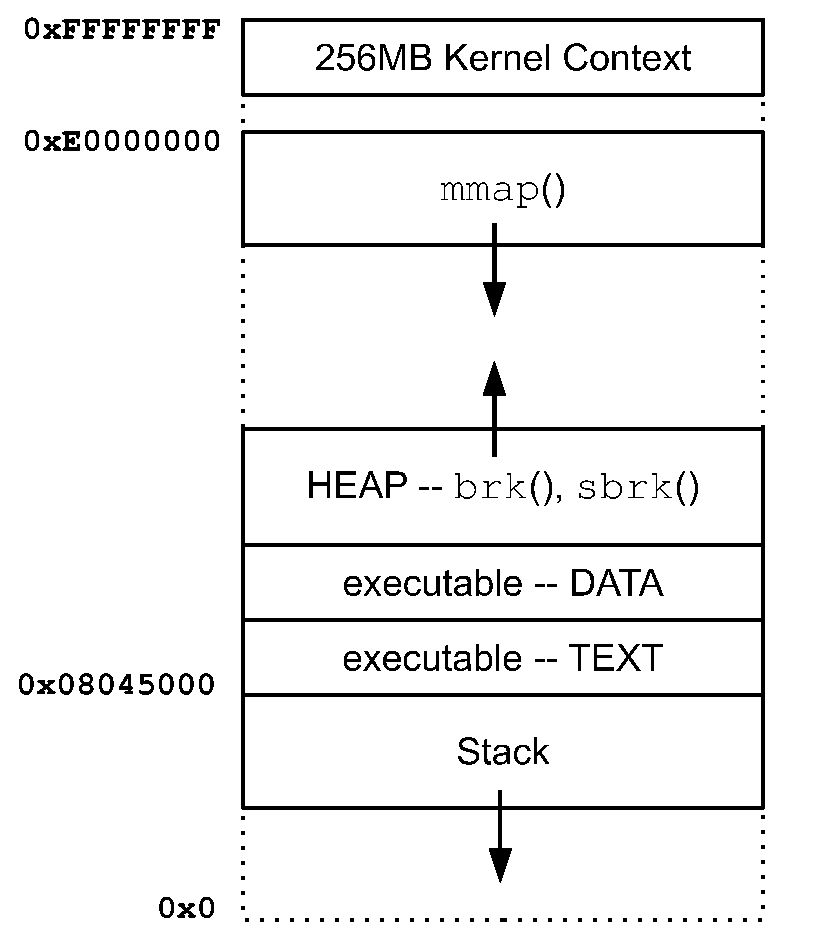
\includegraphics[width=54mm]{img/eps/x86-memory-proc-mem-layout.eps}  
\end{center}
\end{slide}

\label{SOLARIS_PROC_ADDR_SPACE}

\begin{itemize}
\item The following is deductible from the image:

\begin{itemize}
\item maximum size of kernel for Solaris 11 x86 32-bit is 256 megabytes
\item there is free space between kernel and memory reserved for \texttt{mmap}
\item stack grows towards lower addresses and its size is limited to 128 megabytes
\end{itemize}

\item A \emph{heap} is a part of the memory that can be extended by processes
using the \texttt{brk} and \texttt{sbrk} syscalls and is used by the
\texttt{malloc} function.  The \texttt{malloc} allocator gradually extends the
heap on demand, and manages acquired memory and distributes it to the process in
chunks.  When \texttt{free} is called, it does not mean that the memory is
returned to the kernel; it is only returned to the allocator.
\item The \texttt{mmap} area is used for mapping files into memory, i.e. also
for shared libraries. Some allocators use also this memory internally,
e.g. in case a process requests larger chunks of memory at once.  It is possible
to exclusively use just \texttt{mmap}, and that is transparent to the
application. When using \texttt{mmap} it is possible to return the memory to the
kernel (using \texttt{munmap}), in contrast to the \texttt{brk}/\texttt{sbrk}
based implementation.
\item The picture was taken from [McDougall-Mauro] and does not contain space
for non-initialized variables. If you try to print the address of such a
variable on this system, you will find out that both initialized and
non-initialized variables share a common data segment, labeled in the image as
,,executable -- DATA''.  Example: \example{pmap/proc-addr-space.c}.
\item The kernel mapping is not necessary, for example on Solaris running on
\emph{\texttt{amd64}} architecture (i.e. 64-bit) the kernel is no longer mapped
into user space.
\item \texttt{brk} nor \texttt{sbrk} are part of the standard, hence portable
applications should not use them; if a similar functionality is needed, they
should use \texttt{mmap}, see page \pageref{MMAP}.
\end{itemize}

%%%%%

\begin{slide}
\sltitle{Process memory layout in kernel}
\begin{center}
\begin{picture}(0,0)%
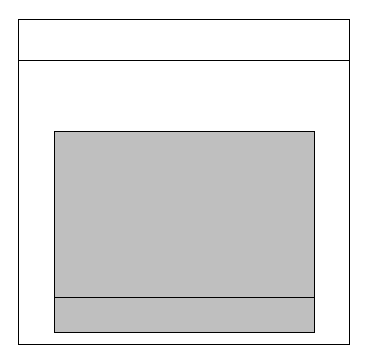
\includegraphics{img/tex/mem_kernel}%
\end{picture}%
\setlength{\unitlength}{4144sp}%
%
\begingroup\makeatletter\ifx\SetFigFont\undefined%
\gdef\SetFigFont#1#2#3#4#5{%
  \reset@font\fontsize{#1}{#2pt}%
  \fontfamily{#3}\fontseries{#4}\fontshape{#5}%
  \selectfont}%
\fi\endgroup%
\begin{picture}(2544,2499)(1339,-1873)
\put(2281,434){\makebox(0,0)[lb]{\smash{\SetFigFont{10}{12.0}{\sfdefault}{\mddefault}{\updefault}{\color[rgb]{0,0,0}kernel text}%
}}}
\put(2071,119){\makebox(0,0)[lb]{\smash{\SetFigFont{10}{12.0}{\sfdefault}{\mddefault}{\updefault}{\color[rgb]{0,0,0}kernel data and bss}%
}}}
\put(1681,-76){\makebox(0,0)[lb]{\smash{\SetFigFont{10}{12.0}{\sfdefault}{\mddefault}{\updefault}{\color[rgb]{0,0,0}(fd tables, variables, etc.)}%
}}}
\put(2138,-466){\makebox(0,0)[lb]{\smash{\SetFigFont{10}{12.0}{\sfdefault}{\mddefault}{\updefault}{\color[rgb]{0,0,0}\texttt{user} struct}%
}}}
\put(2041,-661){\makebox(0,0)[lb]{\smash{\SetFigFont{10}{12.0}{\sfdefault}{\mddefault}{\updefault}{\color[rgb]{0,0,0}of running process}%
}}}
\put(1666,-1411){\makebox(0,0)[lb]{\smash{\SetFigFont{10}{12.0}{\ttdefault}{\mddefault}{\updefault}{\color[rgb]{0,0,0}extern struct user u;}%
}}}
\put(2123,-1681){\makebox(0,0)[lb]{\smash{\SetFigFont{10}{12.0}{\sfdefault}{\mddefault}{\updefault}{\color[rgb]{0,0,0}kernel stack}%
}}}
\end{picture}

\end{center}
\end{slide}

\begin{itemize}
\item A process will enter a kernel model either by a
\emph{trap induced by the CPU} (page fault, unknown instruction, etc.)
\emph{timer} (to invoke scheduler), \emph{interrupt} from a peripheral device,
or synchronous trap (a standard library uses it to hand over the control to
the kernel to service a \emph{system call}).
\item There is only one copy of the kernel text and data in the memory,
shared by all processes. The kernel text as a whole is resident in memory and
not swapped out to disk.
\item \emph{kernel text} \dots{} code of the operating system kernel,
loaded when the system is booting up and is always resident in memory.
Some implementations allow to add modules to the kernel during runtime
(e.g. when a device is connected, matching device driver module is
automatically loaded), it is therefore not necessary to regenerate
the kernel and reboot the system whenever a change is needed.
\item \emph{data and kernel \texttt{bss}} \dots{} contain data structures used
by the kernel, contains the u-area of a currently running process.
\item \emph{kernel stack} \dots{} independent for each process, is empty
when the process is in the user mode (and therefore uses the user stack).
\end{itemize}

%%%%%

\pdfbookmark[1]{segments - text/data/stack}{memsegments}

\begin{slide}
\sltitle{Process memory segments}
\begin{center}
\begin{picture}(0,0)%
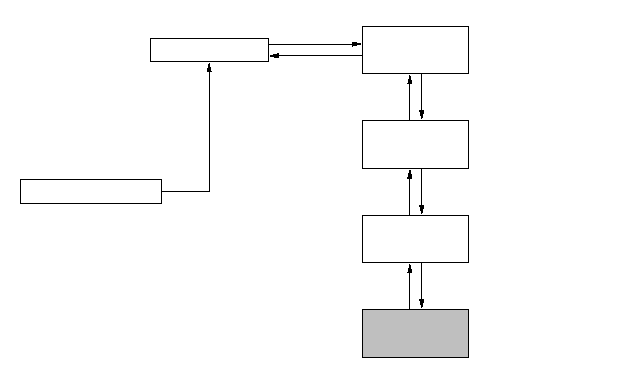
\includegraphics{img/tex/segments}%
\end{picture}%
\setlength{\unitlength}{4144sp}%
%
\begingroup\makeatletter\ifx\SetFigFont\undefined%
\gdef\SetFigFont#1#2#3#4#5{%
  \reset@font\fontsize{#1}{#2pt}%
  \fontfamily{#3}\fontseries{#4}\fontshape{#5}%
  \selectfont}%
\fi\endgroup%
\begin{picture}(4467,2595)(79,-2053)
\put(2791,344){\makebox(0,0)[lb]{\smash{\SetFigFont{10}{12.0}{\sfdefault}{\mddefault}{\updefault}{\color[rgb]{0,0,0}read only}%
}}}
\put(2881,164){\makebox(0,0)[lb]{\smash{\SetFigFont{10}{12.0}{\sfdefault}{\mddefault}{\updefault}{\color[rgb]{0,0,0}shared}%
}}}
\put(181,-826){\makebox(0,0)[lb]{\smash{\SetFigFont{10}{12.0}{\ttdefault}{\mddefault}{\updefault}{\color[rgb]{0,0,0}struct proc}%
}}}
\put(1171,254){\makebox(0,0)[lb]{\smash{\SetFigFont{10}{12.0}{\ttdefault}{\mddefault}{\updefault}{\color[rgb]{0,0,0}struct as}%
}}}
\put(2071,434){\makebox(0,0)[lb]{\smash{\SetFigFont{10}{12.0}{\ttdefault}{\mddefault}{\updefault}{\color[rgb]{0,0,0}a\_segs}%
}}}
\put(2971,-106){\makebox(0,0)[rb]{\smash{\SetFigFont{10}{12.0}{\ttdefault}{\mddefault}{\updefault}{\color[rgb]{0,0,0}s\_prev}%
}}}
\put(2881,-556){\makebox(0,0)[lb]{\smash{\SetFigFont{10}{12.0}{\sfdefault}{\mddefault}{\updefault}{\color[rgb]{0,0,0}private}%
}}}
\put(2791,-1096){\makebox(0,0)[lb]{\smash{\SetFigFont{10}{12.0}{\sfdefault}{\mddefault}{\updefault}{\color[rgb]{0,0,0}read/write}%
}}}
\put(2881,-1276){\makebox(0,0)[lb]{\smash{\SetFigFont{10}{12.0}{\sfdefault}{\mddefault}{\updefault}{\color[rgb]{0,0,0}private}%
}}}
\put(2791,-1816){\makebox(0,0)[lb]{\smash{\SetFigFont{10}{12.0}{\sfdefault}{\mddefault}{\updefault}{\color[rgb]{0,0,0}read/write}%
}}}
\put(2881,-1996){\makebox(0,0)[lb]{\smash{\SetFigFont{10}{12.0}{\sfdefault}{\mddefault}{\updefault}{\color[rgb]{0,0,0}shared}%
}}}
\put(2791,-376){\makebox(0,0)[lb]{\smash{\SetFigFont{10}{12.0}{\sfdefault}{\mddefault}{\updefault}{\color[rgb]{0,0,0}read/write}%
}}}
\put(3241,-106){\makebox(0,0)[lb]{\smash{\SetFigFont{10}{12.0}{\ttdefault}{\mddefault}{\updefault}{\color[rgb]{0,0,0}s\_next}%
}}}
\put(3691,254){\makebox(0,0)[lb]{\smash{\SetFigFont{10}{12.0}{\sfdefault}{\mddefault}{\updefault}{\color[rgb]{0,0,0}text}%
}}}
\put(3691,-466){\makebox(0,0)[lb]{\smash{\SetFigFont{10}{12.0}{\sfdefault}{\mddefault}{\updefault}{\color[rgb]{0,0,0}data}%
}}}
\put(3691,-1186){\makebox(0,0)[lb]{\smash{\SetFigFont{10}{12.0}{\sfdefault}{\mddefault}{\updefault}{\color[rgb]{0,0,0}stack}%
}}}
\put(3691,-1906){\makebox(0,0)[lb]{\smash{\SetFigFont{10}{12.0}{\sfdefault}{\mddefault}{\updefault}{\color[rgb]{0,0,0}shared memory}%
}}}
\put(2206,119){\makebox(0,0)[lb]{\smash{\SetFigFont{10}{12.0}{\ttdefault}{\mddefault}{\updefault}{\color[rgb]{0,0,0}s\_as}%
}}}
\put(4546,-1726){\makebox(0,0)[rb]{\smash{\SetFigFont{10}{12.0}{\ttdefault}{\mddefault}{\updefault}{\color[rgb]{0,0,0} }%
}}}
\end{picture}

\end{center}
\end{slide}

\begin{itemize}
\item This is how memory segments representation looks like in the kernel.
\item The core feature of this architecture is a \emph{memory object}, a
mapping abstraction between a part of memory and a place where data is normally
stored (so called \emph{backing store} or \emph{data object}). This place can
be e.g. swap space or a file. Address space of a process is a set of mappings to
different data objects. There exists also an \emph{anonymous object} that does
not have persistent backing store (it is used e.g. for a stack). Physical memory
then serves as a cache for data of these mapped objects.
\item This coarsely described architecture is called VM (\emph{Virtual
Memory}), and was introduced in SunOS 4.0. The virtual memory architecture
of SVR4 is based on this architecture.  More information can be found in
[Vahalia], the original white paper from 1987 that introduced this architecture:
Gingell, R. A., Moran J.  P., Shannon, W.  A. -- \emph{Virtual Memory
Architecture in SunOS}.
\item To determine what memory segments a memory space of a process consists of,
various tools can be used: \texttt{pmap(1)} on Solaris, NetBSD and in some Linux
distributions, \texttt{procmap(1)} on OpenBSD, or \texttt{vmmap(1)} on macOS.
\end{itemize}

%%%%%

\pdfbookmark[1]{virtual memory}{virtmem}

\begin{slide}
\sltitle{Virtual memory}
\begin{center}
\begin{picture}(0,0)%
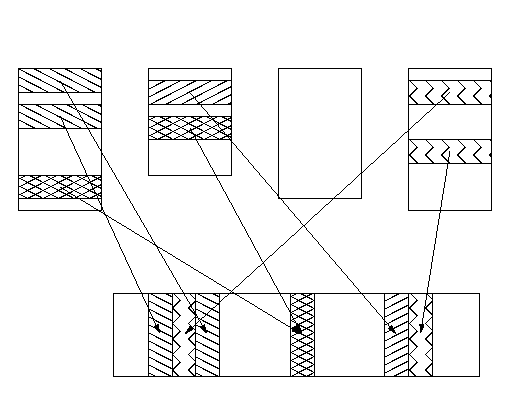
\includegraphics{img/tex/virt_mem}%
\end{picture}%
\setlength{\unitlength}{4144sp}%
%
\begingroup\makeatletter\ifx\SetFigFont\undefined%
\gdef\SetFigFont#1#2#3#4#5{%
  \reset@font\fontsize{#1}{#2pt}%
  \fontfamily{#3}\fontseries{#4}\fontshape{#5}%
  \selectfont}%
\fi\endgroup%
\begin{picture}(3624,2742)(259,-2053)
\put(1621,569){\makebox(0,0)[b]{\smash{\SetFigFont{10}{12.0}{\sfdefault}{\mddefault}{\updefault}{\color[rgb]{0,0,0}process 2}%
}}}
\put(1621,374){\makebox(0,0)[b]{\smash{\SetFigFont{10}{12.0}{\sfdefault}{\mddefault}{\updefault}{\color[rgb]{0,0,0}memory}%
}}}
\put(2611,569){\makebox(0,0)[b]{\smash{\SetFigFont{10}{12.0}{\sfdefault}{\mddefault}{\updefault}{\color[rgb]{0,0,0}process 3}%
}}}
\put(2611,374){\makebox(0,0)[b]{\smash{\SetFigFont{10}{12.0}{\sfdefault}{\mddefault}{\updefault}{\color[rgb]{0,0,0}memory}%
}}}
\put(3601,569){\makebox(0,0)[b]{\smash{\SetFigFont{10}{12.0}{\sfdefault}{\mddefault}{\updefault}{\color[rgb]{0,0,0}process 4}%
}}}
\put(3601,374){\makebox(0,0)[b]{\smash{\SetFigFont{10}{12.0}{\sfdefault}{\mddefault}{\updefault}{\color[rgb]{0,0,0}memory}%
}}}
\put(631,569){\makebox(0,0)[b]{\smash{\SetFigFont{10}{12.0}{\sfdefault}{\mddefault}{\updefault}{\color[rgb]{0,0,0}process 1}%
}}}
\put(631,374){\makebox(0,0)[b]{\smash{\SetFigFont{10}{12.0}{\sfdefault}{\mddefault}{\updefault}{\color[rgb]{0,0,0}memory}%
}}}
\put(901,-1681){\makebox(0,0)[rb]{\smash{\SetFigFont{10}{12.0}{\sfdefault}{\mddefault}{\updefault}{\color[rgb]{0,0,0}physical}%
}}}
\put(901,-1876){\makebox(0,0)[rb]{\smash{\SetFigFont{10}{12.0}{\sfdefault}{\mddefault}{\updefault}{\color[rgb]{0,0,0}memory}%
}}}
\end{picture}

\end{center}
\end{slide}

\begin{itemize}
\item Each process sees its own address space as a contiguous interval of
(virtual) addresses from zero to some maximal value.  Accessible addresses
are those for which there is a mapping, i.e. there is a memory
segment (see the previous slide).
\item The kernel divides the memory to pages. Each page has its own location in
physical memory. This location is determined by kernel page tables and the
memory pages can be arbitrarily mixed w.r.t. their placement in the virtual
address space of a process.
\item If a page is not used it can be swapped out to disk.
\item The kernel memory management ensures a mapping between virtual addresses
used by processes and the kernel to physical addresses.  It also reads in pages
from a disk upon a page fault.
\end{itemize}

%%%%%

\pdfbookmark[1]{Process states}{procstates}

\begin{slide}
\sltitle{Process states}
\begin{center}
\begin{picture}(0,0)%
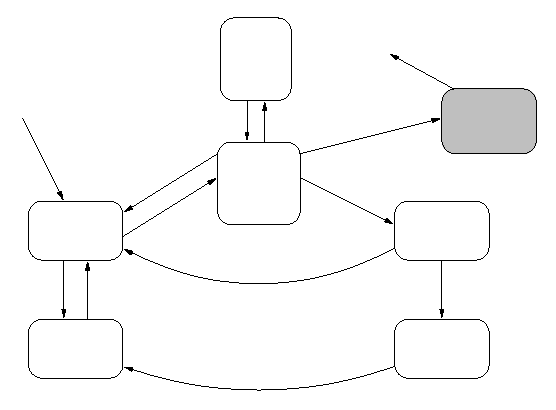
\includegraphics{img/tex/process_states}%
\end{picture}%
\setlength{\unitlength}{4144sp}%
%
\begingroup\makeatletter\ifx\SetFigFont\undefined%
\gdef\SetFigFont#1#2#3#4#5{%
  \reset@font\fontsize{#1}{#2pt}%
  \fontfamily{#3}\fontseries{#4}\fontshape{#5}%
  \selectfont}%
\fi\endgroup%
\begin{picture}(3972,2859)(541,-2053)
\put(2363,614){\makebox(0,0)[b]{\smash{\SetFigFont{10}{12.0}{\sfdefault}{\mddefault}{\updefault}{\color[rgb]{0,0,0}running}%
}}}
\put(2363,419){\makebox(0,0)[b]{\smash{\SetFigFont{10}{12.0}{\sfdefault}{\mddefault}{\updefault}{\color[rgb]{0,0,0}in user}%
}}}
\put(2363,224){\makebox(0,0)[b]{\smash{\SetFigFont{10}{12.0}{\sfdefault}{\mddefault}{\updefault}{\color[rgb]{0,0,0}mode}%
}}}
\put(2386,-331){\makebox(0,0)[b]{\smash{\SetFigFont{10}{12.0}{\sfdefault}{\mddefault}{\updefault}{\color[rgb]{0,0,0}running}%
}}}
\put(2386,-526){\makebox(0,0)[b]{\smash{\SetFigFont{10}{12.0}{\sfdefault}{\mddefault}{\updefault}{\color[rgb]{0,0,0}in kernel}%
}}}
\put(2386,-721){\makebox(0,0)[b]{\smash{\SetFigFont{10}{12.0}{\sfdefault}{\mddefault}{\updefault}{\color[rgb]{0,0,0}mode}%
}}}
\put(3781,-781){\makebox(0,0)[b]{\smash{\SetFigFont{10}{12.0}{\sfdefault}{\mddefault}{\updefault}{\color[rgb]{0,0,0}sleeping}%
}}}
\put(3781,-976){\makebox(0,0)[b]{\smash{\SetFigFont{10}{12.0}{\sfdefault}{\mddefault}{\updefault}{\color[rgb]{0,0,0}in memory}%
}}}
\put(3781,-1681){\makebox(0,0)[b]{\smash{\SetFigFont{10}{12.0}{\sfdefault}{\mddefault}{\updefault}{\color[rgb]{0,0,0}sleeping}%
}}}
\put(3781,-1876){\makebox(0,0)[b]{\smash{\SetFigFont{10}{12.0}{\sfdefault}{\mddefault}{\updefault}{\color[rgb]{0,0,0}on disk}%
}}}
\put(991,-781){\makebox(0,0)[b]{\smash{\SetFigFont{10}{12.0}{\sfdefault}{\mddefault}{\updefault}{\color[rgb]{0,0,0}ready}%
}}}
\put(991,-976){\makebox(0,0)[b]{\smash{\SetFigFont{10}{12.0}{\sfdefault}{\mddefault}{\updefault}{\color[rgb]{0,0,0}in memory}%
}}}
\put(991,-1681){\makebox(0,0)[b]{\smash{\SetFigFont{10}{12.0}{\sfdefault}{\mddefault}{\updefault}{\color[rgb]{0,0,0}ready}%
}}}
\put(991,-1876){\makebox(0,0)[b]{\smash{\SetFigFont{10}{12.0}{\sfdefault}{\mddefault}{\updefault}{\color[rgb]{0,0,0}on disk}%
}}}
\put(4141, 74){\makebox(0,0)[b]{\smash{\SetFigFont{10}{12.0}{\sfdefault}{\mddefault}{\updefault}{\color[rgb]{0,0,0}zombie}%
}}}
\put(4141,-121){\makebox(0,0)[b]{\smash{\SetFigFont{10}{12.0}{\sfdefault}{\mddefault}{\updefault}{\color[rgb]{0,0,0}}%
}}}
\put(541,389){\makebox(0,0)[b]{\smash{\SetFigFont{10}{12.0}{\sfdefault}{\mddefault}{\updefault}{\color[rgb]{0,0,0}inception}%
}}}
\put(3241,659){\makebox(0,0)[b]{\smash{\SetFigFont{10}{12.0}{\sfdefault}{\mddefault}{\updefault}{\color[rgb]{0,0,0}termination}%
}}}
\put(541, 29){\makebox(0,0)[b]{\smash{\SetFigFont{41}{49.2}{\sfdefault}{\mddefault}{\updefault}{\color[rgb]{0,0,0}*}%
}}}
\put(1846,-331){\makebox(0,0)[rb]{\smash{\SetFigFont{10}{12.0}{\sfdefault}{\mddefault}{\updefault}{\color[rgb]{0,0,0}preemption}%
}}}
\put(1621,-1006){\makebox(0,0)[lb]{\smash{\SetFigFont{10}{12.0}{\sfdefault}{\mddefault}{\updefault}{\color[rgb]{0,0,0}CPU}%
}}}
\put(1531,-871){\makebox(0,0)[lb]{\smash{\SetFigFont{10}{12.0}{\sfdefault}{\mddefault}{\updefault}{\color[rgb]{0,0,0}assignment}%
}}}
\put(1171,-1321){\makebox(0,0)[lb]{\smash{\SetFigFont{10}{12.0}{\sfdefault}{\mddefault}{\updefault}{\color[rgb]{0,0,0}load}%
}}}
\put(3871,-1321){\makebox(0,0)[lb]{\smash{\SetFigFont{10}{12.0}{\sfdefault}{\mddefault}{\updefault}{\color[rgb]{0,0,0}swap out}%
}}}
\put(811,-1321){\makebox(0,0)[rb]{\smash{\SetFigFont{10}{12.0}{\sfdefault}{\mddefault}{\updefault}{\color[rgb]{0,0,0}swap out}%
}}}
\put(2386,-1411){\makebox(0,0)[b]{\smash{\SetFigFont{10}{12.0}{\sfdefault}{\mddefault}{\updefault}{\color[rgb]{0,0,0}wakeup}%
}}}
\put(2386,-1951){\makebox(0,0)[b]{\smash{\SetFigFont{10}{12.0}{\sfdefault}{\mddefault}{\updefault}{\color[rgb]{0,0,0}wakeup}%
}}}
\put(2971,-511){\makebox(0,0)[lb]{\smash{\SetFigFont{10}{12.0}{\sfdefault}{\mddefault}{\updefault}{\color[rgb]{0,0,0}put to sleep}%
}}}
\put(2521,-61){\makebox(0,0)[lb]{\smash{\SetFigFont{10}{12.0}{\sfdefault}{\mddefault}{\updefault}{\color[rgb]{0,0,0}return}%
}}}
\put(2206,-61){\makebox(0,0)[rb]{\smash{\SetFigFont{10}{12.0}{\sfdefault}{\mddefault}{\updefault}{\color[rgb]{0,0,0}trap}%
}}}
\put(3511,164){\makebox(0,0)[rb]{\smash{\SetFigFont{10}{12.0}{\ttdefault}{\mddefault}{\updefault}{\color[rgb]{0,0,0}exit}%
}}}
\put(3466,-16){\makebox(0,0)[rb]{\smash{\SetFigFont{10}{12.0}{\ttdefault}{\mddefault}{\updefault}{\color[rgb]{0,0,0}kill}%
}}}
\put(3241,479){\makebox(0,0)[b]{\smash{\SetFigFont{14}{16.8}{\sfdefault}{\mddefault}{\updefault}{\color[rgb]{0,0,0}$\dagger$}%
}}}
\put(3736,389){\makebox(0,0)[lb]{\smash{\SetFigFont{10}{12.0}{\ttdefault}{\mddefault}{\updefault}{\color[rgb]{0,0,0}wait}%
}}}
\end{picture}

\end{center}
\end{slide}

\begin{itemize}
\item After the process is terminated either using an \texttt{exit} call or as a
consequence of a signal, it will transition to a zombie state as the kernel
needs to store a return value for the process. The whole memory of the process is
freed, the only remaining piece is the \texttt{proc} structure. The process can
go away for good only after its parent will retrieve its return value using the
\texttt{wait} call. If the original parent is no longer available, the
\texttt{init} process which became the new parent will call \texttt{wait}.
\item In today's Unix systems processes are usually not swapped out as whole,
only individual pages are.
\item A process is put to sleep if it requests it, e.g. when it is waiting on a
completion of an operation with a peripheral device. The \emph{preemption} is on
the other hand an involuntary removal of a CPU by the scheduler.
\end{itemize}

%%%%%

\begin{slide}
\sltitle{Process scheduling}
\begin{itemize}
\item \emph{preemptive} -- if a process does not give up CPU
(e.g. by entering a sleep to wait on some event), the CPU is taken away
after a time quantum expiration.
\item processes are classified into queues according to a priority,
a CPU is assigned to the first ready process from the queue with the biggest
priority.
\item SVR4 introduced priority queues and real-time support with guaranteed
maximal response time
\item contrary to the previous versions, in SVR4 a bigger number means a bigger
priority
\end{itemize}
\end{slide}

\begin{itemize}
\item \emsl{The premise of preemptive planning are periodic timer interrupts}
which take away the CPU from the running process and pass on the CPU
to the kernel (scheduler is activated).
\item The other variant is non-preemptive (cooperative) planning, where process
keeps running, until it gives up the CPU, i.e. until it calls such system call,
that switches the context to different process. The downside of cooperative
planning is that one process can block the CPU and other processes forever.
\item Unix uses only preemptive planning for user processes.
\item Traditional (historical) UNIX \emsl{kernel} uses cooperative planning,
i.e. process running in kernel mode is not switched until it gives up the CPU
by itself.
\emsl{Modern Unix kernels are preemptive} -- mainly because of real-time
systems; where it is necessary to have the possibility to remove a CPU from
a running process immediately, and not waiting until it returns from a kernel
mode or enters sleep by itself. Note that UNIX was preemptive from its very
beginning but its kernel was non-preemptive in the beginning.
\item With a preemptive planning processes can be interrupted at any time and
the CPU given to another process. Therefore a process can never be sure
that a given operation (spanning more than one instruction, besides system calls
with guaranteed atomicity) will be executed atomically, without being
influenced by other processes. If it is necessary to ensure atomicity of an
operation, processes must synchronize. This problem is avoided in a cooperative
planning -- the atomicity of a given operation is simply ensured by not giving
up the CPU while the operation is still in progress.
\end{itemize}

%%%%%

\pdfbookmark[1]{Priority classes for process scheduling}{prioclasses}

\begin{slide}
\sltitle{Priority classes}
\setlength{\baselineskip}{0.8\baselineskip}
\begin{itemize}
\item \emsl{system}
    \begin{itemize}
    \item priority 60 to 99 
    \item reserved for system processes (\texttt{pageout},
    \texttt{sched}, \dots) 
    \item fixed priority 
    \end{itemize}
\item \emsl{real-time}
    \begin{itemize}
    \item priority 100 to 159 
    \item fixed priority 
    \item a time quantum corresponds to priority value
    \end{itemize}
\item \emsl{time-shared}
    \begin{itemize}
    \item priority 0 to 59 
    \item dynamic 2 part priority, fixed user part and
    dynamic system part -- if a process uses CPU extensively,
    its priority is being decreased (and time quantum increased)
    \end{itemize}
\end{itemize}
\end{slide}

\begin{itemize}
\item The system class is used only by the kernel, a user process running
in a kernel mode retains its own planning characteristics.
\item Processes in the real time class have the biggest priority and so should
be configured correctly otherwise they could block the rest of the system from
getting any CPU time.
\item If a process in a time-shared class is put to sleep and is waiting on an
event, the system priority is temporarily assigned to it.  After a wake-up, such
a process will be assigned a CPU earlier than other non-sleeping processes to
finish the operation as soon as possible as it could hold some locks later
needed by other processes.
\item Fixed part of the priority in the time-shared class can be set using\\
ifdef([[[NOSPELLCHECK]]], [[[
\texttt{int \funnm{setpriority}(int \emph{which}, id\_t \emph{who},
int \emph{prio});}\\ or \\ \texttt{int \funnm{nice}(int \emph{in{}cr});} \\
]]])
The \emph{which} value determines what will be in the \emph{who} argument.
If \emph{which} is e.g. \emph{\texttt{PRIO\_PGRP}}, the \emph{who} will store
process group number.  Note that \funnm{nice} call will return a new nice value.
As -1 is a valid value, it is necessary to clear \texttt{errno} and then check
if the function returns -1.
\item The priority class and nice value of a given process can be displayed with
the \texttt{-l} option of the \texttt{ps} command or by explicitly specifying
the fields to be printed out (see the \texttt{-o} option).
\item Example: priority values have different scales on different systems.  E.g.
on macOS~10.9 a process that had the priority value 30 will have the value
decremented to 21 after increasing the nice value:
\begin{verbatim}
$ sleep 200 &
[1] 36877
$ ps -O pri,nice -p $!
  PID PRI NI   TT  STAT      TIME COMMAND
36877  31  0 s003  S      0:00.00 sleep 200
$ renice 10 -p $!
$ ps -O pri,nice -p $!
  PID PRI NI   TT  STAT      TIME COMMAND
36877  21 10 s003  SN     0:00.00 sleep 200
\end{verbatim}

With Linux kernel 3.10 it will look differently -- the priority value will be
increased after a nice value increases.  However, that means the process will be
running with a smaller priority.
\end{itemize}

%%%%%

\pdfbookmark[1]{process groups}{procgrps}

\begin{slide}
\sltitle{Process groups, controlling terminals}
\begin{itemize}
\item every process belongs to a \emph{process group}
\item each group can have a leading process, so called \emph{group leader}
\item every process can have a \emph{controlling terminal} (usually it is a
login terminal)
\item special file \texttt{/dev/tty} is associated with a controlling terminal
of each process
\item each terminal is associated with a process group called a
\emph{controlling group}
\item \emph{job control} is a mechanism for suspending, resuming, and
terminating process groups and control their access to terminals
\item \emph{session} is a collection of process groups created for the purpose
of job control
\end{itemize}
\end{slide}

\begin{itemize}
\item When a user logs into a system, a new session is created.  The session
contains one process group that only has a single process -- one with the user's
shell.  That process is also the leader of that single process group and also a
session leader.  In case a job control is on, each command or a pipeline will
create a new process group, and one process from each group will always become a
process group leader.  One of the groups can be running in the foreground, the
rest will be running in the background.  Signals which are generated from the
keyboard (i.e. those triggered by combination of keys, not by executing the
\texttt{kill} command) are sent only to the group running in the foreground.
\item If the job control is off, command execution in the background means that
the shell will not be waiting for its completion.  There exists only one group of
processes, and keyboard generated signals are sent to all processes running in
the foreground and background.  Processes cannot be moved to the background from
the foreground and ifdef([[[NOSPELLCHECK]]], [[[vice versa]]]).
\item When a process that has a controlling terminal opens the \texttt{/dev/tty}
file, it gets associated with its controlling terminal, i.e. if two different
processes open this file, each will be accessing a different terminal.
\item In bash a process group (job) can be stopped temporarily using
\texttt{Ctrl-Z}, and can be resumed again using ,,\texttt{fg \%N}'' where
\texttt{N} is the number from the \texttt{jobs} command listing.  More
information can be found in the ``JOB CONTROL'' section in the bash man page.
\end{itemize}

\pdfbookmark[1]{fork}{fork}

\begin{slide}
\sltitle{Create a new process: \texttt{fork()}}
\begin{center}
\begin{picture}(0,0)%
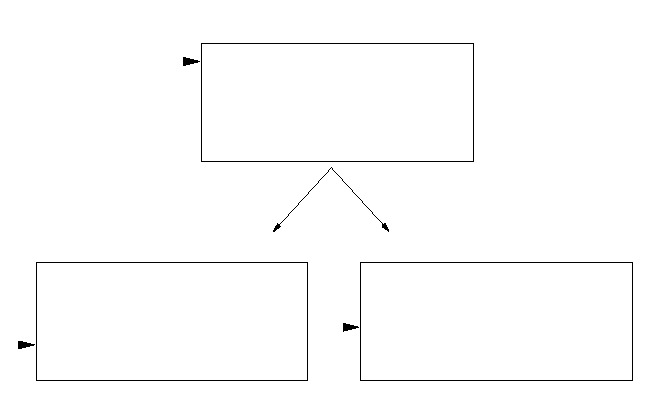
\includegraphics{img/tex/fork}%
\end{picture}%
\setlength{\unitlength}{4144sp}%
%
\begingroup\makeatletter\ifx\SetFigFont\undefined%
\gdef\SetFigFont#1#2#3#4#5{%
  \reset@font\fontsize{#1}{#2pt}%
  \fontfamily{#3}\fontseries{#4}\fontshape{#5}%
  \selectfont}%
\fi\endgroup%
\begin{picture}(4705,2775)(33,-2008)
\put(226,-1575){\makebox(0,0)[lb]{\smash{\SetFigFont{10}{8.0}{\ttdefault}{\mddefault}{\updefault}{\color[rgb]{0,0,0}
\begin{minipage}{4.5cm}switch(pid = fork()) \{\\
\mbox{}\ \ \ \ case -1: /* Chyba */\\
\mbox{}\ \ \ \ case\ \ 0: /* D�t�\ \ */\\
\mbox{}\ \ \ \ \emprg{default: /* Rodi� */}\\
\}\end{minipage}}%
}}}
\put(2701,-1575){\makebox(0,0)[lb]{\smash{\SetFigFont{10}{8.0}{\ttdefault}{\mddefault}{\updefault}{\color[rgb]{0,0,0}%
\begin{minipage}{4.5cm}switch(pid = fork()) \{\\
\mbox{}\ \ \ \ case -1: /* Chyba */\\
\mbox{}\ \ \ \ \emprg{case\ \ 0: /* D�t�\ \ */}\\
\mbox{}\ \ \ \ default: /* Rodi� */\\
\}\end{minipage}}%
}}}
\put(181,-1006){\makebox(0,0)[lb]{\smash{\SetFigFont{10}{12.0}{\ttdefault}{\mddefault}{\updefault}{\color[rgb]{0,0,0}getpid()==1234, pid==2345}%
}}}
\put(1441,659){\makebox(0,0)[lb]{\smash{\SetFigFont{10}{12.0}{\ttdefault}{\mddefault}{\updefault}{\color[rgb]{0,0,0}getpid() == 1234}%
}}}
\put(2656,-1006){\makebox(0,0)[lb]{\smash{\SetFigFont{10}{12.0}{\ttdefault}{\mddefault}{\updefault}{\color[rgb]{0,0,0}getpid()==2345, pid==0}%
}}}
\put(2791,-691){\makebox(0,0)[lb]{\smash{\SetFigFont{10}{12.0}{\sfdefault}{\mddefault}{\updefault}{\color[rgb]{0,0,0}d�t� (nov� proces)}%
}}}
\put(2071,-691){\makebox(0,0)[rb]{\smash{\SetFigFont{10}{12.0}{\sfdefault}{\mddefault}{\updefault}{\color[rgb]{0,0,0}rodi� (pokra�uje)}%
}}}
\put(1486,90){\makebox(0,0)[lb]{\smash{\SetFigFont{10}{8.0}{\ttdefault}{\mddefault}{\updefault}{\color[rgb]{0,0,0}
\begin{minipage}{4.5cm}switch(\emprg{pid = fork()}) \{\\
\mbox{}\ \ \ \ case -1: /* Chyba */\\
\mbox{}\ \ \ \ case\ \ 0: /* D�t�\ \ */\\
\mbox{}\ \ \ \ default: /* Rodi� */\\
\}\end{minipage}}%
}}}
\end{picture}

\end{center}
\end{slide}

\begin{itemize}
\item \label{FORK} The child process is almost an exact copy of its parent
except for the following:
\begin{itemize}
\item The child process has a unique process and parent process ID.
\item If the parent had multiple threads, the child will only have one that
called \texttt{fork}; will be further explained on page \pageref{FORKALL}.
\item Child process resource utilization counters are set to 0.
\item \texttt{alarm} settings and file locks are not inherited.
\end{itemize}
\item The file descriptor tables are exact copies in both processes.  That means
that more processes can share and seek a common file position.  Signal masks are
not changed, more on that on page \pageref{SIGNALBLOCKINGEXAMPLE}.
\item For efficiency and less memory consumption, the address space is not copied
but a \emph{copy-on-write} mechanism is used.
\item The reason why the parent gets its child's PID as a return value and the
child gets 0 is because it is easy for the child to get its parent PID via
\texttt{getpid}.  Imagine how the parent would figure out the new child PID,
especially if it already spawned multiple children.
\item Example: \example{fork/fork.c}
\item \label{VFORK} There is also \texttt{vfork}, used in the past to work
around the problem that the child address space was usually rewritten on
subsequent \texttt{exec}.  This problem was solved via already mentioned
copy-on-write mechanism.  See \example{fork/vfork.c} on how it works.
\item The problems of \texttt{vfork} are largely solved by
\texttt{posix\_spawn}. See page \pageref{SPAWN}.
\end{itemize}

%%%%%

ifdef([[[NOSPELLCHECK]]], [[[
\pdfbookmark[1]{getpid, getpgrp, getppid, getsid}{getp}
]]])

\begin{slide}
\sltitle{Process identification}
ifdef([[[NOSPELLCHECK]]], [[[
\texttt{pid\_t \funnm{getpid}(void);}
]]])
\begin{itemize}
\item returns the process ID of the calling process.
\end{itemize}
ifdef([[[NOSPELLCHECK]]], [[[
\texttt{pid\_t \funnm{getpgrp}(void);}
]]])
\begin{itemize}
\item returns the PGID of the calling process
\end{itemize}
ifdef([[[NOSPELLCHECK]]], [[[
\texttt{pid\_t \funnm{getppid}(void);}
]]])
\begin{itemize}
\item returns the process ID of the parent process.
\end{itemize}
ifdef([[[NOSPELLCHECK]]], [[[
\texttt{pid\_t \funnm{getsid}(pid\_t \emph{pid});}
]]])
\begin{itemize}
\item returns the session ID for process \texttt{pid} (0 means for the calling
process)
\end{itemize}
\end{slide}

\begin{description}
\item[process groups] make it possible to send signals to group of processes
at once
\item[session] is a collection of processes created for (\emph{job control}).

The processes of the session share one \emph{controlling terminal}.
Session includes one or more process groups. Maximum one group in the session
runs in foreground (\emph{foreground process group}) and has access to the
controlling terminal for input and output, the rest is running in the background
(\emph{background process groups}) and have only optional access to the output
or no at all. (disallowed operation with terminal will stop the process).
\item[parent process:] Each process (besides \texttt{swapper},
\texttt{pid~==~0})
has a parent, i.e. process that created it with the \texttt{fork} syscall.
If the parent exits before the child, its adoptive parent will become the
\texttt{init} process, that will take care of the zombie after the process ends.
\end{description}
\begin{itemize}
\item To get information about running processes programmatically is possible
using non-standard API (e.g. the \texttt{libproc} library on Solaris built
on top of the \texttt{procfs} filesystem that is mounted under \texttt{/proc}).
\item Note that using \texttt{getppid} value to check if parent exited is not
portable (commonly \texttt{init} has \texttt{pid} 1 however this is not true in
many virtualized/containerized environments, e.g. in PID namespaces on Linux,
Zones in Solaris).\\
Example: \example{session/getppid.c}.
\end{itemize}


%%%%

ifdef([[[NOSPELLCHECK]]], [[[
\pdfbookmark[1]{setpgrp, setsid}{setp}
]]])

\begin{slide}
\sltitle{Creating a new process group/session}
ifdef([[[NOSPELLCHECK]]], [[[
\texttt{int \funnm{setpgid}(pid\_t \emph{pid}, pid\_t \emph{pgid});}
]]])
\begin{itemize}
\item sets the PGID of the process specified by \texttt{pid} to \texttt{pgid}.
\end{itemize}
ifdef([[[NOSPELLCHECK]]], [[[
\texttt{pid\_t \funnm{setsid}(void);}
]]])
\begin{itemize}
\item creates a new session if the calling process is not a process
group leader
\end{itemize}
\end{slide}

\begin{itemize}
\item For the \funnm{setpgid} syscall the following is true:
\begin{enumerate}
\item ifdef([[[NOSPELLCHECK]]], [[[pid == pgid]]]) : the process with
\emph{\texttt{pid}} will become process group leader
\item ifdef([[[NOSPELLCHECK]]], [[[pid != pgid]]]) : the process with
\emph{\texttt{pid}} will become process group member
\end{enumerate}
\item The process which is not yet process group leader can both become session
leader and process group leader using \texttt{setsid}. If the process already is
process group leader, \texttt{setsid} will fail. To overcome this it is necessary
to call \texttt{fork} and call \texttt{setsid} in the child process.
Such process does not have controlling terminal however it can acquire it by
opening a terminal which is not yet controlling terminal of a session when
\texttt{open} flags argument does not contain the \texttt{O\_NOCTTY} flag,
or using other implementation dependent way.
\end{itemize}

%%%%%

%%%%%

\pdfbookmark[1]{exec}{exec}

\begin{slide}
\sltitle{Execute a program: \texttt{exec}}
ifdef([[[NOSPELLCHECK]]], [[[
\texttt{extern char **\funnm{environ};\\
int \funnm{execl}(const char *\emph{path}, const char *\emph{arg0}, ... );}
]]])
\begin{itemize}
\item replaces the current process image with a new process image
\item runs a program defined via \emph{path}
\item arguments that follow, including \emph{\texttt{arg0}}, are given to the
program via \texttt{argc} and \texttt{argv} of its \texttt{main()}
\item the argument list must end with \texttt{(char *)0}, i.e. \texttt{NULL}
\item \emph{\texttt{arg0}} should contain the program name (i.e. not the full
path)
\item \emsl{open file descriptors are unaffected by \funnm{exec}}
\begin{itemize}
\item \dots{}aside from file descriptors with flag \texttt{FD\_CLOEXEC}
\end{itemize}
\end{itemize}
\end{slide}

\label{EXEC}

\begin{itemize}
\item \emph{path} must be an absolute or relative path to the executable file.
\texttt{PATH} is only used for \funnm{execlp} a \funnm{execvp} (see the one of
the slides that follow), if \emph{path} does not contain \texttt{'/'}.
\item All variants of these calls are commonly just called the \funnm{exec}
call.  It goes without saying that one of the variants is used but usually that
is not important for the sake of a discussion.
\item Sometimes \texttt{argv[0]} is different from the executable file name.
For example, \texttt{login} command prefixes the shell file name with
\texttt{'-'}, e.g. \texttt{-bash}.  The shell then knows it is supposed to
function as a login shell.  A login shell reads \texttt{/etc/profile}, for
example.
\item \funnm{exec} does not transfer the control to the program in memory
directly. As described on page \pageref{RUNTIMELINKER}, the system (i.e. the
code of the \funnm{exec} call) first maps the dynamic linker, aka loader, to the
process address space.  The loader then maps all dynamic libraries there as
well, then finally calls the program \texttt{main()}.
\item A useful exercise is to write a simple program calling \texttt{open()},
for example.  When done, run the program via \texttt{truss(1)} or
\texttt{strace(1)} like this: \texttt{truss ./a.out}. You will see what is being
done before \texttt{open} is called in the end.
\end{itemize}

\begin{slide}
\sltitle{Execute a program: \texttt{exec} (continued)}
ifdef([[[NOSPELLCHECK]]], [[[
\texttt{extern char **\funnm{environ};\\
int \funnm{execl}(const char *\emph{path}, const char *\emph{arg0}, ... );}
]]])
\begin{itemize}
\item successful \funnm{execl} never returns as the new process (program) fully
replaced the address space of the calling process
\begin{itemize}
\item ...the original place to return to no longer exists
\end{itemize}
\item signal handlers are set to default
\begin{itemize}
\item ...as the original handler code no longer exists
\end{itemize}
\item the new process inherits \texttt{environ} from the calling process
\end{itemize}
\end{slide}

\begin{itemize}
\item More about signals on page \pageref{SIGNALS}.
\item \funnm{exec} does not change RUID and RGID.  And for security reasons, if
the executed program has a SUID bit set, the program's EUID and saved EUID are
set to the UID of the executable program owner.
\item Today's systems can also execute scripts that start with a line:\\
\texttt{\#!/\emph{interpreter\_path}/\emph{interpreter\_name} \emph{[args]}}
\end{itemize}

%%%%%

ifdef([[[NOSPELLCHECK]]], [[[
\pdfbookmark[1]{execv, execle, execl, execve, execlp}{execvariants}
]]])

\begin{slide}
\sltitle{Variants of the \texttt{exec} call}
\setlength{\baselineskip}{0.8\baselineskip}
\texttt{int \funnm{execv}(const char *\emph{path}, char *const \emph{argv}[]);} 
\begin{itemize}
\item like \funnm{execl} but arguments are in the \emph{argv} array,
the last item must be \texttt{NULL}
\end{itemize}
\begin{minipage}{\slidewidth}
ifdef([[[NOSPELLCHECK]]], [[[
\vspace{-1ex}\texttt{\begin{tabbing}
int \funnm{execle}(\=const char *\emph{path}, const char *\emph{arg0},
... ,\\\> char *const \emph{envp}[]);
\end{tabbing}}
]]])
\end{minipage}
\begin{itemize}
\item like \funnm{execl} but instead of the global variable \emph{environ}, 
the \emph{\texttt{envp}} argument is used
\end{itemize}
\begin{minipage}{\slidewidth}
ifdef([[[NOSPELLCHECK]]], [[[
\vspace{-1ex}\texttt{\begin{tabbing}
int \funnm{execve}(\=const char *\emph{path}, char *const \emph{argv}[],\\
\>char *const \emph{envp}[]);
\end{tabbing}}
]]])
\end{minipage}
\begin{itemize}
\item like \funnm{execv} but instead of \emph{\texttt{environ}},
\emph{\texttt{envp}} is used
\end{itemize}
ifdef([[[NOSPELLCHECK]]], [[[
\texttt{int \funnm{execlp}(const char *\emph{file}, const char *\emph{arg0},
...);\\
int \funnm{execvp}(const char *\emph{file}, char *const \emph{argv}[]);}
]]])
\begin{itemize}
\item like \funnm{execl} and \funnm{execv} but \texttt{PATH} is also used
for searching for the executable file
\end{itemize}
\end{slide}

\begin{itemize}
\item \emsl{l} = list (i.e. list of arguments), \emsl{v} = vector (i.e.  an array
of string pointers), \emsl{e}~=~environment (i.e. environment variables are
passed to the function via an argument), \emsl{p} = \texttt{PATH} is used.
\item Aside from \funnm{execlp} and \funnm{execvp}, it is always needed to use
the full path to the executable program, either an absolute or relative one.
\item All variants aside from \funnm{execle} and \funnm{execve}
are also passing to the program being executed the environment variables of the
calling process, i.e. the \texttt{environ} array.
\item For some unknown historical reasons, there is no ``p'' with ``e'' together
in the standard.  However, GNU provides \funnm{execvpe} as an extension.
\item \label{EXEC_DATE} Example: \example{exec/exec-date.c}
\item \label{EXECL} The following use of \funnm{execl} is incorrect as it is
missing the mandatory argument for \texttt{argv[0]}:

\begin{verbatim}
	execl("/bin/ls", NULL);
\end{verbatim}

On some systems, the above has very interesting consequences.  As \texttt{NULL}
is taken as an expected \texttt{argv[0]}, the data on the stack are then
accepted as the program arguments until the next \texttt{NULL} is found there.
In the following example, run on some version of the FreeBSD system, \texttt{ls}
is trying to list file names that are environment variable names and values (the
environment array contain strings \texttt{<varname>=<value>}), as those were on
the stack because the environment was passed to the program being executed, as
we already know.  In my case, the output was:

\begin{verbatim}
$ ./a.out 
: BLOCKSIZE=K: No such file or directory
: FTP_PASSIVE_MODE=YES: No such file or directory
: HISTCONTROL=ignoredups: No such file or directory
: HISTSIZE=10000: No such file or directory
...
...
\end{verbatim}

\end{itemize}

%%%%%

\pdfbookmark[1]{ELF}{ELF}

\begin{slide}
\sltitle{Executable file format}
\begin{itemize}
\item \emsl{a.out} format, in early UNIX versions
\item \emsl{Common Object File Format (COFF)} -- AT\&T System V, superseded
\emsl{a.out}
\item \emsl{Extensible Linking Format (ELF)} -- new in SVR4, replaced both older
formats
\item ELF format:\quad
\raisetab{\begin{tabular}[t]{|c|}
\hline
ELF header\\
\hline
\quad \quad program header table \quad\quad \\
\hline
section 1\\
\hline
$\vdots$\\
\hline
section N\\
\hline
section header table\\
\hline
\end{tabular}}
\end{itemize}
\end{slide}

\label{ELF}

\begin{itemize}
\item The UNIX standard does not specify what executable file format systems
should use.  While most of the UNIX and Unix-like systems (e.g. Linux
distributions) use ELF, there are other widely used systems that do not. One
example is macOS (which is a certified UNIX system) that uses the \emph{Mach-O}
file format, short for \emph{Mach Object}. Each Mach-O file is made
up of one Mach-O header, followed by a series of load commands, followed by one
or more segments, each of which contains between 0 and 255 sections.
\item On Solaris, the \texttt{elfdump} command allows listing sections of the
ELF file in a human readable form. On Linux distributions, use \texttt{readelf}.
\item The \emph{ELF header} contains basic information about the file.  Try
``\texttt{readelf -h /bin/ls}'' on any Linux distribution.
\item The \emph{program header table} is only present in files that are
executable.  For example, dynamic libraries are ELF files that are not
executable.  It contains information on the virtual memory layout.  You can list
the table via ``\texttt{elfdump~-p}'' or ``\texttt{readelf~-l}''.
\item Sections contain code, data, symbol table, relocation data, etc.
\item The \emph{section header table} contains information for the linker, see
``\texttt{elfdump -c}'' or ``\texttt{readelf~-S}''.
\item Some systems stuck on a format based on the original \emph{a.out} for a
long time.  For example, OpenBSD moved from \emph{a.out} to ELF in 2003 when
releasing version 3.4.
\item Today it is common that systems randomly arrange the address space
positions of key data areas of a process, including the base of the executable
and the positions of the stack, heap and libraries.  This technique is called
\emph{Address Space Layout Randomization} (ASLR) and its objective is to prevent
an attacker from reliably jumping to, for example, a particular exploited
function in memory.  First introduced as a Linux kernel patch.  OpenBSD was the
first mainstream operating system to support ASLR by default, in version 3.4,
released in 2003.  Different systems apply this technique with different
parameters and on different parts of a program.  In general it is possible to
introduce randomness into other parts of a system, for example process IDs,
initial TCP sequence numbers, etc.
\end{itemize}

%%%%%

ifdef([[[NOSPELLCHECK]]], [[[
\pdfbookmark[1]{exit, wait, waitpid}{procexit}
]]])

\begin{slide}
\sltitle{Program termination}
\setlength{\baselineskip}{0.6\baselineskip}
ifdef([[[NOSPELLCHECK]]], [[[
\texttt{void \funnm{exit}(int \emph{status});}
]]])
\begin{itemize}
\item terminates a process with a return value \emph{status}.  Never returns.
\end{itemize}
ifdef([[[NOSPELLCHECK]]], [[[
\texttt{pid\_t \funnm{wait}(int *\emph{stat\_loc});}
]]])
\begin{itemize}
\item waits for a child process termination, returns its PID and puts
termination information into \emph{\texttt{stat\_loc}} which can be tested as:
    \begin{itemize}
    \item \texttt{WIFEXITED(stat\_loc)} \dots{} process called
    \texttt{exit()}
    \item \texttt{WEXITSTATUS(stat\_loc)} \dots{} argument of
    \texttt{exit()}
    \item \texttt{WIFSIGNALED(stat\_loc)} \dots{} process got a signal
    \item \texttt{WTERMSIG(stat\_loc)} \dots{} signal number
    \item \texttt{WIFSTOPPED(stat\_loc)} \dots{} process stopped
    (\texttt{WUNTRACED} flag required, need \funnm{waitpid} below)
    \item \texttt{WSTOPSIG(stat\_loc)} \dots{} stop signal number
    \end{itemize}
\end{itemize}
ifdef([[[NOSPELLCHECK]]], [[[
\texttt{pid\_t \funnm{waitpid}(pid\_t \emph{pid}, int *\emph{stat\_loc},
int \emph{opts});}
]]])
\begin{itemize}
\item waits for a specific child process termination
\end{itemize}
\end{slide}

\begin{itemize}
\item \emph{\texttt{status\_loc}} equal to \texttt{NULL} means to ignore the
status information.
\item Function \funnm{\_exit} works as \funnm{exit} but it does not flush stdio
streams and functions registered with the \funnm{atexit} call are not called.
\item There is also \texttt{WIFCONTINUED(stat\_loc)} which means a restarted
process after having been stopped before.  However, it is part of an extension
that not all systems support.
\item You can stop a process using ``\texttt{kill -STOP <PID>}'',
and restart it with ''\texttt{kill -CONT <PID>}''.
\item \emph{opts} in \funnm{waitpid} are an OR combination of the following
flags:
    \begin{itemize}
    \item \texttt{WNOHANG} \dots{} does not hang if there are no processes
    that wish to report status
    \item \texttt{WUNTRACED} \dots{} children of the current process that were
    stopped due to a \texttt{SIGTTIN}, \texttt{SIGTTOU}, \texttt{SIGTSTP}, or
    \texttt{SIGSTOP} signal also have their status reported.  Such processes are
    reported only once per such a situation.
    \item \texttt{WCONTINUED} \dots{} also report children of the current
    process that were restarted after having been stopped (and not waited for
    yet).  Part of the same extension as \texttt{WIFCONTINUED}.
    \item For the \texttt{WUNTRACED} and \texttt{WCONTINUED} flags, you should
    only use them in portable code if a macro \texttt{\_POSIX\_JOB\_CONT\-ROL}
    is defined in \texttt{<unistd.h>}.
    \end{itemize}
\item \emph{\texttt{pid}} in \funnm{waitpid}:
    \begin{itemize}
    \item \texttt{== -1} \dots{} wait for any child
    \item \texttt{> 0} \dots{} wait for a specific child
    \item \texttt{== 0} \dots{} wait for any child in the same process group as
    the calling process
    \item \texttt{< -1} \dots{} wait for any child in the process group of
    \texttt{abs(pid)}
    \end{itemize}
\item There are also \funnm{wait3} and \funnm{wait4} calls. These are more
generic versions, also allowing to gather resource utilization statistics from
exited child.
\item A parent should always call one of the wait functions otherwise the system
will accumulate \emph{zombies} -- terminated processes that occupy process table
slots only to be waited for by their parents.  Zombies could eventually exhaust
all the system memory.  Note that if the parent exits, its children are adopted
by the \texttt{init} process that will call \funnm{wait} on such processes.
However, you should always use wait for children even if you know the parent
will exit soon.
\item Actually, you could notify the system that the program will not wait for
its children in which case such zombies will not accumulate.  See page
\pageref{IGNORE_SIG_CHLD}.
\end{itemize}

%%%%%

\begin{slide}
\sltitle{Example: start a new process and wait}
\begin{center}
\begin{picture}(0,0)%
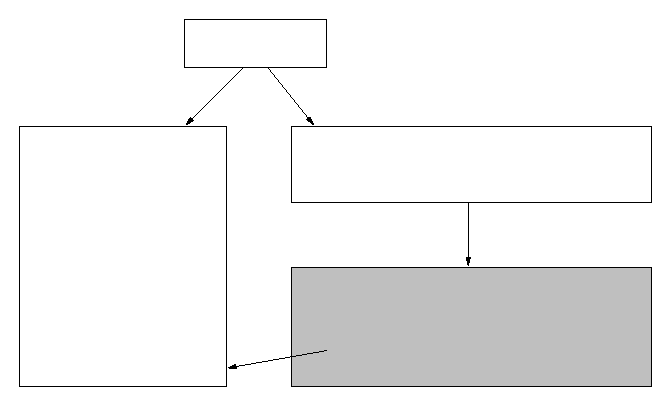
\includegraphics{img/tex/fork_wait}%
\end{picture}%
\setlength{\unitlength}{4144sp}%
%
\begingroup\makeatletter\ifx\SetFigFont\undefined%
\gdef\SetFigFont#1#2#3#4#5{%
  \reset@font\fontsize{#1}{#2pt}%
  \fontfamily{#3}\fontseries{#4}\fontshape{#5}%
  \selectfont}%
\fi\endgroup%
\begin{picture}(4839,2814)(-101,-2053)
\put(1216,614){\makebox(0,0)[lb]{\smash{\SetFigFont{10}{12.0}{\ttdefault}{\mddefault}{\updefault}{\color[rgb]{0,0,0}int status;}%
}}}
\put(1216,449){\makebox(0,0)[lb]{\smash{\SetFigFont{10}{12.0}{\ttdefault}{\mddefault}{\updefault}{\color[rgb]{0,0,0}pid = \emprg{fork()}}%
}}}
\put(2116,119){\makebox(0,0)[lb]{\smash{\SetFigFont{10}{12.0}{\sfdefault}{\mddefault}{\updefault}{\color[rgb]{0,0,0}d�t�}%
}}}
\put(1306,119){\makebox(0,0)[rb]{\smash{\SetFigFont{10}{12.0}{\sfdefault}{\mddefault}{\updefault}{\color[rgb]{0,0,0}rodi�}%
}}}
\put(2026,-1276){\makebox(0,0)[lb]{\smash{\SetFigFont{10}{12.0}{\ttdefault}{\mddefault}{\updefault}{\color[rgb]{0,0,0}int main(int argc, char *argv[])}%
}}}
\put(2026,-1456){\makebox(0,0)[lb]{\smash{\SetFigFont{10}{12.0}{\ttdefault}{\mddefault}{\updefault}{\color[rgb]{0,0,0}\{}%
}}}
\put(2026,-1636){\makebox(0,0)[lb]{\smash{\SetFigFont{10}{12.0}{\ttdefault}{\mddefault}{\updefault}{\color[rgb]{0,0,0}\ \ \ \ ...}%
}}}
\put(2026,-1801){\makebox(0,0)[lb]{\smash{\SetFigFont{10}{12.0}{\ttdefault}{\mddefault}{\updefault}{\color[rgb]{0,0,0}\ \ \ \ \emprg{exit}(result);}%
}}}
\put(2026,-1966){\makebox(0,0)[lb]{\smash{\SetFigFont{10}{12.0}{\ttdefault}{\mddefault}{\updefault}{\color[rgb]{0,0,0}\}}%
}}}
\put(2026,-1051){\makebox(0,0)[lb]{\smash{\SetFigFont{10}{12.0}{\ttdefault}{\mddefault}{\updefault}{\color[rgb]{0,0,0}/bin/ls}%
}}}
\put(2026,-196){\makebox(0,0)[lb]{\smash{\SetFigFont{10}{12.0}{\ttdefault}{\mddefault}{\updefault}{\color[rgb]{0,0,0}else}%
}}}
\put(2026,-361){\makebox(0,0)[lb]{\smash{\SetFigFont{10}{12.0}{\ttdefault}{\mddefault}{\updefault}{\color[rgb]{0,0,0}\ \ \ \ \emprg{execl}("/bin/ls",}%
}}}
\put(2026,-556){\makebox(0,0)[lb]{\smash{\SetFigFont{10}{12.0}{\ttdefault}{\mddefault}{\updefault}{\color[rgb]{0,0,0}\ \ \ \ \ \ \ \ \ \ "ls", "/", NULL);}%
}}}
\put(-44,-196){\makebox(0,0)[lb]{\smash{\SetFigFont{10}{12.0}{\ttdefault}{\mddefault}{\updefault}{\color[rgb]{0,0,0}if(pid > 0)}%
}}}
\put(-44,-1951){\makebox(0,0)[lb]{\smash{\SetFigFont{10}{12.0}{\ttdefault}{\mddefault}{\updefault}{\color[rgb]{0,0,0}\ \ \ \ \emprg{wait}(\&status);}%
}}}
\end{picture}

\end{center}
\end{slide}

\begin{itemize}
\item This is a typical way to start a new process and continue after its
termination.  The parent could also choose not to wait for the child termination
right away but carry on with its life and wait for the child later.
\item Note that you have to use macros from the previous slide to get the
child's return value out of the status information.
\item \label{WAITPID} Example: \example{wait/wait.c}
\item \label{SPAWN} Creating new process with \texttt{fork} and replacing the
process address space etc. with a new one after \texttt{exec} has been done is
expensive and has other problems. To make kernel create new process directly
from executable \texttt{posix\_spawn} can be used.
Example: \example{exec/spawn.c}
\end{itemize}

%%%%%

\label{PIPEREADWRITE}

\pdfbookmark[1]{pipe}{pipe}

\begin{slide}
\sltitle{\texttt{pipe()}}
\texttt{int \funnm{pipe}(int \emph{fildes}[2]);}
\begin{itemize}
\item creates an unnamed pipe and allocates a pair of file descriptors
    \begin{itemize}
    \item \texttt{fildes[0]} \dots{} reading from a pipe
    \item \texttt{fildes[1]} \dots{} writing to a pipe
    \end{itemize}
\item the system makes sure that:
    \begin{itemize}
    \item producer blocks on writing if the pipe is full
    \item consumer blocks on reading if the pipe is empty
    \end{itemize}
\item consumer gets \texttt{EOF} (i.e. \texttt{read()} returns
\texttt{0}) only if all copies of \texttt{fildes[1]} are closed.
\item named pipe (i.e. FIFO, see \funnm{mkfifo}) works the same way.  The
difference is any process can use it.
\end{itemize}
\end{slide}

\label{PIPE}

\begin{itemize}
\item An unnamed pipe is created by one process and can be passed to its
children only via file descriptors inherited through \funnm{fork}.  That
limitation can be worked around via passing an open file descriptor via a
u{}nix-domain socket.  However, such a workaround is out of scope for this
class.
\item If the function \funnm{write} writes at most \texttt{PIPE\_BUF} bytes to
the pipe, it is guaranteed that the write will be atomic, i.e. such bytes will
not be intermingled with bytes written by other producers.
\item \label{TWO_WAY_PIPES} The SUSv3 standard does not specify whether
\texttt{fildes[0]} is also open for writing and if \texttt{fildes[1]} is also
open for reading.  FreeBSD and Solaris provide bidirectional pipes while Linux
may not.  It is best to assume unidirectional pipes.
\item \emsl{Important:} the same rules applied to reading and writing from/to
named pipes stand for unnamed pipes as well, see page \pageref{NAMEDPIPE}.
\item Example: \example{pipe/broken-pipe.c}, \example{pipe/deadlock-in-read.c}
\end{itemize}

%%%%%

\begin{slide}
\sltitle{Example: a pipe between two processes}
\begin{center}
\begin{picture}(0,0)%
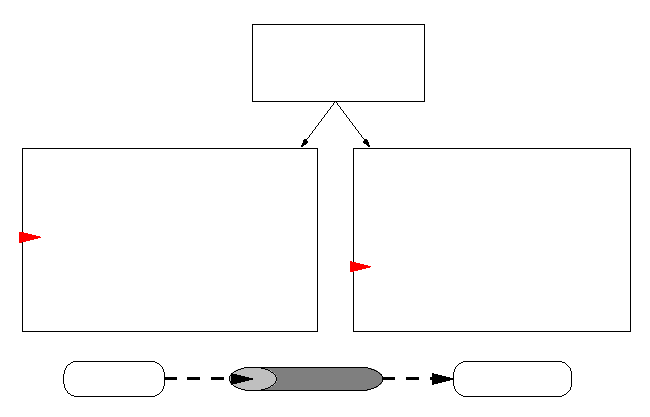
\includegraphics{img/tex/pipe}%
\end{picture}%
\setlength{\unitlength}{4144sp}%
%
\begingroup\makeatletter\ifx\SetFigFont\undefined%
\gdef\SetFigFont#1#2#3#4#5{%
  \reset@font\fontsize{#1}{#2pt}%
  \fontfamily{#3}\fontseries{#4}\fontshape{#5}%
  \selectfont}%
\fi\endgroup%
\begin{picture}(4686,2892)(7,-2098)
\put( 91,659){\makebox(0,0)[lb]{\smash{\SetFigFont{10}{12.0}{\sfdefault}{\mddefault}{\updefault}{\color[rgb]{0,0,0}shell:}%
}}}
\put( 91,-331){\makebox(0,0)[lb]{\smash{\SetFigFont{8}{9.6}{\ttdefault}{\mddefault}{\updefault}{\color[rgb]{0,0,0}case 0:}%
}}}
\put( 91,-526){\makebox(0,0)[lb]{\smash{\SetFigFont{8}{9.6}{\ttdefault}{\mddefault}{\updefault}{\color[rgb]{0,0,0}\ \ \emprg{close}(1);}%
}}}
\put( 91,-916){\makebox(0,0)[lb]{\smash{\SetFigFont{8}{9.6}{\ttdefault}{\mddefault}{\updefault}{\color[rgb]{0,0,0}\ \ \emprg{close}(pd[0]);}%
}}}
\put( 91,-1111){\makebox(0,0)[lb]{\smash{\SetFigFont{8}{9.6}{\ttdefault}{\mddefault}{\updefault}{\color[rgb]{0,0,0}\ \ close(pd[1]);}%
}}}
\put( 91,-1306){\makebox(0,0)[lb]{\smash{\SetFigFont{8}{9.6}{\ttdefault}{\mddefault}{\updefault}{\color[rgb]{0,0,0}\ \ execl("/bin/ls", "ls",}%
}}}
\put( 91,-1501){\makebox(0,0)[lb]{\smash{\SetFigFont{8}{9.6}{\ttdefault}{\mddefault}{\updefault}{\color[rgb]{0,0,0}\ \ \ \ \ \ \ \ "/", NULL);}%
}}}
\put(3106,-106){\makebox(0,0)[lb]{\smash{\SetFigFont{10}{12.0}{\sfdefault}{\mddefault}{\updefault}{\color[rgb]{0,0,0}konzument (rodi�)}%
}}}
\put(676,-106){\makebox(0,0)[lb]{\smash{\SetFigFont{10}{12.0}{\sfdefault}{\mddefault}{\updefault}{\color[rgb]{0,0,0}producent (d�t�)}%
}}}
\put(1261,-1771){\makebox(0,0)[lb]{\smash{\SetFigFont{10}{12.0}{\ttdefault}{\mddefault}{\updefault}{\color[rgb]{0,0,0}pd[1]}%
}}}
\put(2701,-1771){\makebox(0,0)[lb]{\smash{\SetFigFont{10}{12.0}{\ttdefault}{\mddefault}{\updefault}{\color[rgb]{0,0,0}pd[0]}%
}}}
\put(3421,-1996){\makebox(0,0)[lb]{\smash{\SetFigFont{10}{12.0}{\ttdefault}{\mddefault}{\updefault}{\color[rgb]{0,0,0}/bin/more}%
}}}
\put(1846,614){\makebox(0,0)[lb]{\smash{\SetFigFont{8}{9.6}{\ttdefault}{\mddefault}{\updefault}{\color[rgb]{0,0,0}int pd[2];}%
}}}
\put(1846,224){\makebox(0,0)[lb]{\smash{\SetFigFont{8}{9.6}{\ttdefault}{\mddefault}{\updefault}{\color[rgb]{0,0,0}switch(fork()) \{}%
}}}
\put(2611,-331){\makebox(0,0)[lb]{\smash{\SetFigFont{8}{9.6}{\ttdefault}{\mddefault}{\updefault}{\color[rgb]{0,0,0}default:}%
}}}
\put(2611,-526){\makebox(0,0)[lb]{\smash{\SetFigFont{8}{9.6}{\ttdefault}{\mddefault}{\updefault}{\color[rgb]{0,0,0}\ \ \emprg{close}(0);}%
}}}
\put(2611,-721){\makebox(0,0)[lb]{\smash{\SetFigFont{8}{9.6}{\ttdefault}{\mddefault}{\updefault}{\color[rgb]{0,0,0}\ \ \emprg{dup}(pd[0]);}%
}}}
\put(2611,-916){\makebox(0,0)[lb]{\smash{\SetFigFont{8}{9.6}{\ttdefault}{\mddefault}{\updefault}{\color[rgb]{0,0,0}\ \ close(pd[0]);}%
}}}
\put(2611,-1111){\makebox(0,0)[lb]{\smash{\SetFigFont{8}{9.6}{\ttdefault}{\mddefault}{\updefault}{\color[rgb]{0,0,0}\ \ \emprg{close}(pd[1]);}%
}}}
\put(2611,-1306){\makebox(0,0)[lb]{\smash{\SetFigFont{8}{9.6}{\ttdefault}{\mddefault}{\updefault}{\color[rgb]{0,0,0}\ \ execl("/bin/more",}%
}}}
\put(2611,-1501){\makebox(0,0)[lb]{\smash{\SetFigFont{8}{9.6}{\ttdefault}{\mddefault}{\updefault}{\color[rgb]{0,0,0}\ \ \ \ \ \ \ \ "more", NULL);}%
}}}
\put(451,-1996){\makebox(0,0)[lb]{\smash{\SetFigFont{10}{12.0}{\ttdefault}{\mddefault}{\updefault}{\color[rgb]{0,0,0}/bin/ls}%
}}}
\put(496,659){\makebox(0,0)[lb]{\smash{\SetFigFont{10}{12.0}{\ttdefault}{\mddefault}{\updefault}{\color[rgb]{0,0,0}ls / | more}%
}}}
\put(1846,419){\makebox(0,0)[lb]{\smash{\SetFigFont{8}{9.6}{\ttdefault}{\mddefault}{\updefault}{\color[rgb]{0,0,0}\emprg{pipe}(pd);}%
}}}
\put( 91,-721){\makebox(0,0)[lb]{\smash{\SetFigFont{8}{9.6}{\ttdefault}{\mddefault}{\updefault}{\color[rgb]{0,0,0}\ \ \emprg{dup}(pd[1]);}%
}}}
\end{picture}

\end{center}
\end{slide}

\label{FDSHARING}

\begin{itemize}
\item Remember, open file descriptors are unaffected by \funnm{exec} aside from
file descriptors with the \texttt{FD\_CLOEXEC} flag -- those are closed in the
\emsl{successful} \funnm{exec} call.
\item Example: \example{pipe/pipe-and-fork.c}
\item Closing the writing descriptor \texttt{pd[1]} (see
ifdef([[[NOSPELLCHECK]]], [[[{\color[rgb]{1,0,0} $\triangleright$}]]]))
in the consumer process is required as the EOF would not be detected otherwise.
\item Closing the reading descriptor \texttt{pd[0]} in the producer process is
desired as well (see
ifdef([[[NOSPELLCHECK]]], [[[{\color[rgb]{1,0,0} $\triangleright$}]]])
) as if the consumer finishes prematurely the producer properly gets a
\texttt{SIGPIPE}.
If that file descriptor in the producer was not closed while the consumer died
in the middle of processing the data, for example, the producer would not learn
that the consumer was gone (as the producer would remain to be an existing
reader itself), and would hang indefinitely on \funnm{write} after filling up
the pipe.
\item If we are not sure that the descriptor \texttt{0} was open before calling
\funnm{pipe}, we have to call \texttt{dup2(pd[1], 1)} in the producer as
otherwise \texttt{dup(pd[1])} could reuse the file descriptor \texttt{0} in
place of expected \texttt{1}.  You might also need to check if \verb#pd[1] == 1#
(i.e. standard output was closed before calling \funnm{pipe}) as in that case we
could actually close one end of the pipe.  Similarly, in the consumer you might
need to check if \verb#pd[0] == 0#.
\item It is better to create a pipe from a child to its parent as typically the
process writing the pipe finishes first, then the consumer reads the rest of the
data, processes it, and then finally exits.  In general, the shell waits for the
program it started, i.e. the parent, and it does not care at all about children
the running program spawned during its life.  If the pipe was created the other
way around, the shell could print the prompt after the parent finished while the
data from the child might still be flowing to the console.  However, nowadays
the shell waits for all processes in the pipeline.  For example, the following
will take 10 seconds before you get the prompt even though \texttt{cat(1)} might
exit right away if \texttt{sleep(1)} closed its standard error before putting
itself to sleep: \texttt{date | sleep 10 | cat}.
\item For example, the original \emph{Bourne shell} constructed a pipeline the
way that the last process created a child as its producer, that producer itself
created its child as its producer, and this continued until the whole pipeline
was formed, i.e. the first command in the pipeline was created as the last
process.
\item However, in \texttt{bash}, all processes in a pipeline are direct children
of the shell itself, i.e. \texttt{bash} calls \funnm{fork} that many times as is
the number of programs in the pipeline.  Before the prompt is printed, it waits
for all processes it directly created to finish.
\end{itemize}

%%%%%

\begin{slide}
\sltitle{Shared memory -- introduction}
\begin{itemize}
\item using pipes and files to communicate between processes requires system
calls
\begin{itemize}
\item pros: processes cannot corrupt address space of one another
\item cons: significant syscall overhead (typically \funnm{read},
\funnm{write})
\end{itemize}
\item \emph{shared memory} means to map a part of memory into an address space
of multiple processes
\item syscall overhead is gone but processes may become dangerous to one another
\item memory access synchronization is needed
\begin{itemize}
  \item System V semaphores
  \item POSIX semaphores
\end{itemize}
\end{itemize}
\end{slide}

\begin{itemize}
\item Memory file mapping is one of the implementations of shared memory.  A
file name is used to describe the shared piece of memory.
\item A memory mapped file is regularly written to disk.
\item Memory based disks and filesystem are provided by today's system.  They
primarily rely on main memory for data storage, thus avoiding overhead of
physical storage reads and writes.
\end{itemize}

%%%%%

ifdef([[[NOSPELLCHECK]]], [[[
\pdfbookmark[1]{mmap}{mmap}
]]])

\begin{slide}
\sltitle{Mapping files to memory (1)}
ifdef([[[NOSPELLCHECK]]], [[[
\begin{minipage}{\slidewidth}\vspace{-1\baselineskip}\texttt{\begin{tabbing}
void *\funnm{mmap}(\=void *\emph{addr}, size\_t \emph{l{}en},
int \emph{prot}, int \emph{flags},\\\> int \emph{fildes}, off\_t \emph{off});
\end{tabbing}}
]]])
\end{minipage}
\begin{itemize}

\item A file section of \emph{l{}en} bytes, starting at position \texttt{off} in
a file represented by a file descriptor \texttt{fildes}, mapped to the process
space starting at address \emph{\texttt{addr}} (\texttt{0} \dots{}kernel assigns
the address).
\item Returns the address of the mapped section, or \texttt{MAP\_FAILED}. 
\item In \emph{\texttt{prot}}, there is an OR combination of \texttt{PROT\_READ}
(read allowed), \texttt{PROT\_WRITE} (write allowed), \texttt{PROT\_EXEC}
(execution allowed), or \texttt{PROT\_NONE} (no access allowed).
\item In \emph{flags} there is an OR combination of \texttt{MAP\_PRIVATE}
(changes private to the process, not saved to the file), and
\texttt{MAP\_SHARED} (modifications are saved to the file)
\end{itemize}
\end{slide}

\label{MMAP}

\begin{itemize}
\setlength{\itemsep}{0.8\itemsep}
\item Examples: \example{mmap/reverse.c}, \example{mmap/map-nocore.c}
\item in the flags \emsl{exactly one} of \texttt{MAP\_PRIVATE},
\texttt{MAP\_SHARED} has to be present.
There is also \texttt{MAP\_FIXED}, with which the
kernel tries to map the section at \emph{\texttt{addr}} even if it means to
destroy already existing mapping.  Without \texttt{MAP\_FIXED}, the kernel
will try to use \emph{\texttt{addr}} but if there is an existing mapping, it
will try to find another address to use (and returns it).
\item mapping files in memory is alternative to processing files using
\texttt{read}, \texttt{write}, \texttt{lseek}.  After the file is mapped it is
possible to work with it as a data structure in memory. The file is not being
copied to the memory as a whole, rather only the pages which are accessed are
allocated. If it is necessary to free some page, the contents are written back
to the storage, i.e. the file. That is, if the \texttt{MAP\_SHARED} is used
-- this way of mapping is therefore equivalent to writing back via
\texttt{write(2)}) or to the swap -- same copy-on-write mechanism is used
(when using \texttt{MAP\_PRIVATE}).
\item For the file to be mapped into memory it is first necessary to open it
via \texttt{open}. The access mode in \texttt{prot} cannot be ``higher'' than
specified in the mode for \texttt{open}.
\item The use of \texttt{MAP\_FIXED} is not recommended, since it hampers
portability of the code.
\item \textbf{warning:} w.r.t. \texttt{MAP\_SHARED} -- if the file is truncated
by another process so that the truncation affects the mapped part, the access
to such area results in the \texttt{SIGBUS} resp. \texttt{SIGSEGV} or signal
to be sent to the process. One way how to get around it is to use
mandatory locking, however it is not implemented in all the systems.
In case the mapped memory is used as a parameter for \texttt{write},
the signal will not be sent and \texttt{write} will return -1
with \texttt{errno} set to \texttt{EFAULT}.
\item when using \texttt{MAP\_PRIVATE} on Solaris all the changes done by other
processes that have mapped the file using \texttt{MAP\_SHARED} are visible
until the process writes to the page.
-- at this moment a copy of the page is created and subsequent changes by
other processes are not visible anymore.
On FreeBSD the changes are not visible even before the first write.
The spec says:
\emph{,,It is unspecified whether modifications to the underlying object done
after the \texttt{MAP\_PRIVATE} mapping is established are visible through the
\texttt{MAP\_PRIVATE} mapping.''}
\item the value of \texttt{off+l{}en} can exceed current size of the file,
however it is not possible to write beyond the end of the file and thus
extend the file - the process would otherwise receive the \texttt{SIGBUS} or
\texttt{SIGSEGV} signal, see example \example{mmap/lseek.c}.
The signal is also received when attempting to write to file mapped read-only.
(this makes sense, the assignment does not have a return value which can be
tested)
\item the mapping is done in whole pages, the \texttt{off} values have to
be aligned correctly (also when using \texttt{MAP\_FIXED} the \texttt{addr}).
Last page after the end of file is padded with zeroes and this section is
never written back to the file.
\item It is possible to share anonymous mapping between processes using
\texttt{fork()}. The only alternative is shared memory established using
\texttt{shmat}.
\item Access to the mapped region beyond the existing page of mapped object
causes \texttt{SIGBUS} or \texttt{SIGSEGV} signal.
This is not universally true, see example \example{mmap/sigbus.c}.
\item When using \texttt{MAP\_FIXED} the new mapping will replace any existing
mapping from \texttt{addr} to
ifdef([[[NOSPELLCHECK]]], [[[\texttt{addr+l{}en-1}]]]), see example
\example{mmap/override.c}.
\item extensions not part of SUSv3:
    \begin{itemize}
    \setlength{\itemsep}{0.8\itemsep}
    \item \texttt{MAP\_ANONYMOUS} flag -- will create anonymous segment
    (without association to a file), the descriptor has to be \texttt{-1}.
    An anonymous object is mapped that has storage in swap area.
    This flag is frequently used by heap allocators.
    see also page \pageref{SOLARIS_PROC_ADDR_SPACE}.
    \item in IRIX it is possible to use \texttt{MAP\_AUTOGROW} that will
    automatically grow mapped object when accessing beyond its current end.
    \end{itemize}
\item Example of system command using file mapping is \texttt{cat(1)}. 
Using mapped memory is more efficient than calling \texttt{read} repeatedly,
saving the overhead necessary for switching to kernel and back to userspace.
\end{itemize}

%%%%%

ifdef([[[NOSPELLCHECK]]], [[[
\pdfbookmark[1]{msync, munmap, mprotect}{msync}
]]])

\begin{slide}
\sltitle{Mapping files to memory (2)}
ifdef([[[NOSPELLCHECK]]], [[[
\texttt{int \funnm{msync}(void *\emph{addr}, size\_t \emph{l{}en},
int \emph{flags});}
]]])
\begin{itemize}
\item will write back specified pages in the region of l{}en bytes from address
\texttt{addr}. The flags is OR-combination of:
    \begin{itemize}
    \item \texttt{MS\_ASYNC} \dots{} asynchronous write
    \item \texttt{MS\_SYNC} \dots{} synchronous write
    \item \texttt{MS\_INVALIDATE} \dots{} destroy mapped data,
    different to file contents
    \end{itemize}
\end{itemize}
ifdef([[[NOSPELLCHECK]]], [[[
\texttt{int \funnm{munmap}(void *\emph{addr}, size\_t \emph{l{}en});}
]]])
\begin{itemize}
\item write back changes, destroy mapping of length \texttt{l{}en} from
address \texttt{addr}.
\end{itemize}
ifdef([[[NOSPELLCHECK]]], [[[
\texttt{int \funnm{mprotect}(void *\emph{addr}, size\_t \emph{l{}en},
int \emph{prot});}
]]])
\begin{itemize}
\item change access rights to mapped section of a file. The values
\texttt{prot} are the same as for \texttt{mmap()}.
\end{itemize}
\end{slide}

\begin{itemize}
\item writing the changes to the storage is guaranteed only after
\texttt{msync} or \texttt{munmap}, however other processes that have the file
mapped as well will see the changes immediately.
\item mapping to memory and setting access rights is used by the
Electric Fence library, which is used for detection of errors when using
dynamic memory.
\end{itemize}


%%%%%

\begin{slide}
\sltitle{Example: mapping files into memory}
\setlength{\baselineskip}{0.8\baselineskip}
\begin{alltt}
int main(int argc, char *argv[])
\{
    int fd, fsz; char *addr, *p1, *p2, c;

    fd = \emprg{open}(argv[1], O\_RDWR);
    fsz = \emprg{lseek}(fd, 0, SEEK\_END);
    p1 = addr = \emprg{mmap}(0, fsz, PROT\_READ|PROT\_WRITE,
                     MAP\_SHARED, fd, 0);
    p2 = p1 + fsz - 1;
    while(p1<p2) \{
        c = *p1; *p1++ = *p2; *p2-- = c;
    \}
    \emprg{munmap}(addr, fsz); 
    \emprg{close}(fd);
    return (0);
\}
\end{alltt}
\end{slide}

\begin{itemize}
\item This program will reverse the bytes in a file.
\item One of the advantages of shared memory segments is that it is possible
to work with the data using pointer arithmetic. Generally it is necessary
to watch out for alignment when dereferencing a pointer, e.g. on SPARC 
unaligned access will cause the \texttt{SIGBUS} signal, see example
\example{mmap/aligned.c}.
\end{itemize}

%%%%%

ifdef([[[NOSPELLCHECK]]], [[[
\pdfbookmark[1]{dlopen, dlsym, dlclose, dlerror}{dynlib}
]]])

\begin{slide}
\sltitle{Accessing dynamic link libraries}
\texttt{void *\funnm{dlopen}(const char *\emph{path}, int \emph{mode});} 
\begin{itemize}
\item loads \emph{path} unless already loaded, returns
a \emsl{handle} or \texttt{NULL}
\item in \emph{mode} there is an OR combination of \texttt{RTLD\_NOW} (immediate
bind), \texttt{RTLD\_LAZY} (bound when needed), \texttt{RTLD\_GLOBAL}
(symbols accessible from all modules), \texttt{RTLD\_LOCAL} (symbols accessible
through the handle only)
\end{itemize}
\texttt{void *\funnm{dlsym}(void *\emph{handle}, const char *\emph{symbol});}
\begin{itemize}
\item returns the address of \emph{symbol}
\end{itemize}
\texttt{int \funnm{dlclose}(void *\emph{handle});}
\begin{itemize}
\item closes the dynamic library
\end{itemize}
\texttt{char *\funnm{dlerror}(void);}
\begin{itemize}
\item gets diagnostic information
\end{itemize}
\end{slide}

\label{DLOPEN}

\begin{itemize}
\item For example, you could use these functions to implement a dynamically
loadable plug-in modules.  Modules to load could be determined either on the fly
based on user input, or could be read from a configuration file.
\item If you have multiple dynamic libraries that all define a symbol of the
same name, you could link one of those during the build process, and other
libraries can be accessed via \funnm{dlopen}.
\item You need a file of a correct format.  For example, on a Linux
distribution, that is an ELF shared library with an \texttt{.so} suffix.  With
\texttt{gcc}, you will need \texttt{-shared} to build such a library there.  If
on macOS (file format \emph{Mach-O}), you will need \texttt{-dynamiclib}.
Libraries there have a \texttt{.dynlib} suffix.
\item If \emph{path} contains \texttt{/}, it is taken either as global or
relative, if not, the dynamic linker uses its default path to search for the
library, usually in \texttt{/lib} and \texttt{/usr/lib}.  You can extend the
list of paths to search via an environment variable \texttt{LD\_LIBRARY\_PATH}.
Be careful when using it, see page \pageref{EVIL_LDLIBPATH}.
\item flags for \emph{mode} of \funnm{dlopen}:
    \begin{itemize}
    \item \texttt{RTLD\_NOW} -- all undefined symbols in the library are
    resolved before \funnm{dlopen} returns. \texttt{NULL} is returned if it
    cannot be done. That is the default.
    \item \texttt{RTLD\_LAZY} -- only resolves symbols as the code that
    references them is executed.  However, references to variables are always
    immediately bound when the library is loaded.  You can force the specific
    behavior via environment variables \texttt{LD\_BIND\_NOW} and
    \texttt{LD\_BIND\_LAZY}.  If there is a conflict, \texttt{NOW} prevails.
    When a program is started, all linked libraries are bound right away unless
    the program or individual libraries are linked for ``lazy binding'' via
    \texttt{-z lazy} (\texttt{gcc}).  See manual pages for \texttt{ld} a
    \texttt{ld.so.1} (Solaris) or \texttt{ld.so} (Linux).  Example:
    \example{dyn-lib/ld-lazy.c}.
    \item \texttt{RTLD\_GLOBAL} \dots{} symbols defined by the shared object
    will be  made available for symbol resolution of subsequently loaded
    objects.  That is the default for objects mapped when executing a program.
    For \funnm{dlopen}, the default is \texttt{RTLD\_LOCAL}.  It means
    the same library can be mapped multiple times via \funnm{dlopen} and the
    symbols in the mapped instances of the same library will not overlap.
    However, all globally mapped symbols from there are shared, e.g.
    \texttt{errno}.
    \end{itemize}
\item \label{RTLD_NEXT} Special handle \texttt{RTLD\_NEXT} searches the symbol
only in libraries loaded after the library that called \funnm{dlsym}.  Handy for
redefining existing functions if we need to call the original function in our
redefined one.  The library with a modified function is loaded first, possibly
using \texttt{LD\_PRELOAD}, and the address of the original function can be
found using
ifdef([[[NOSPELLCHECK]]], [[[
\texttt{dlsym(RTLD\_NEXT, \emph{fn\_name})}.
]]])
Example: \example{dyn-lib/rtld\_next.c}.
\item  All these functions are part of the dynamic linker that each dynamically
linked program has mapped into its address space upon execution.  Also see pages
\pageref{RUNTIMELINKER} and \pageref{EXEC}.
\end{itemize}

%%%%%

\begin{slide}
\sltitle{Example: accessing a dynamic library}
\begin{alltt}
void *handle;
double y, x = 1.3;
double (*fun)(double); 
char *libname = "libm.so", *fn\_name = "sin";

if ((handle = \emprg{dlopen}(libname, RTLD\_NOW)) == NULL)
        err(1, "dlopen: %s", \emprg{dlerror}());

if ((fun = \emprg{dlsym}(handle, fn\_name)) == NULL)
        err(1, "dlsym: %s", \emprg{dlerror}());

y = fun(x);
\emprg{dlclose}(handle);
\end{alltt}
\end{slide}

\begin{itemize}
\item The code calls function \funnm{sin} from \texttt{libm.so}, the math
library.
\item \funnm{dlsym} returns the symbol address but always as a pointer to
\texttt{void}, there is no type check, and no type information is available
either.  The caller must retype the returned address.
\item If you use C++, note that \emph{name mangling} is used.
\item Example: \example{dyn-lib/dlopen.c}
\end{itemize}

\endinput
